\section{Introduction}
    Executing computational services on the cloud provides certain advantages \cite{microsoft_corporation_what_nodate}, like scaling, performance and speed. However, it also brings some inconvenience, for instance: (i) additional latency to the sending and reception of the data, (ii) the high energetic consumption, (iii) the downtime of the services which could happen even if the vendor assures a "four nines" (99,99\%) uptime availability. There is an alternative to this situation, the usage of edge devices which conforms the edge layer.
        
    \subsection{Motivation for Heterogeneous Computing}
        Traditional homogeneous systems have been decaying at speed of light as opposed to heterogeneous systems, which have been on the rise in the past few years and will prevail. Nowadays, there are a number of compelling reasons as for moving toward heterogeneous environments:
        
        \textbf{Tailored nodes}
        
        The adoption of diversity in cluster makes it possible to have diverse tailored nodes for different computing needs.
        
        \textbf{Resources usage optimization}
        
        Different devices make different resources available. Using these wisely will result in better computation efficiency, better throughput and lower energetic footprint \cite{mittal_survey_2015}.
        
        In light of the above, this newer approach explores and exploits its computational capabilities, bringing computation power to a higher limit. However, it also brings some technical difficulties and challenges along, these will be discussed in the next section.

    \subsection{The complexity of heterogeneity and its challenges}
        Each heterogeneous device from a distributed system can have different characteristics. Consequently, it can be concluded that for a system to be heterogeneous adds one more dimension of difficulty to deploy an application in it.
    
        \subsubsection{Hardware Challenges}
            Among many hardware challenges \cite{mittal_survey_2015, zahran_heterogeneous_2017}, there are a few that should be taken into consideration:
            
            \begin{enumerate}
                \item Types of Processing Units: CPU, GPU, TPU, etc
                \item Processing Unit specific:
                    \begin{itemize}
                        \item Architecture of Heterogeneous Computing Systems (Unified or Discrete)
                        \item Current load on PUs and achieving load balancing between them.
                        \item Memory bandwidth and PUs data transfer overhead.
                    \end{itemize}
                
                \item The memory hierarchy: Usually, the memory hierarchy plays a big role in the performance of a computer system. There is a need to engineer a robust architecture to support heterogeneous cores accesses and optimize the requirements of each. There is also a heterogeneity in these memories since different memories use unalike storage technologies (for caches [SRAM], volatile memory [DRAM], non-volatile memory[Flash, STT-RAM, PCM, etc]) \cite{meena_overview_2014}.
 
                    \begin{itemize}
                        \item Processing Unit's internal storage: Processors' registers \& cache. These memories access times \cite{mistretta_microns_nodate} are around <1nS to a couple of ten nS, depending on the type. Heterogeneity in memory and data storage types:
                        
                            \begin{itemize}
                                \item Registers: <1nS
                                \item L1 Cache Access: 0,9nS
                                \item L2 Cache Access: 2,8nS
                                \item L3 Cache Access: 12,9nS
                            \end{itemize}
                        
                        \item System main storage:
                            \begin{itemize}
                                \item RAM memory Access: 120nS
                            \end{itemize}
                        \item System secondary storage:
                        \begin{itemize}
                            \item Solid-State Disk: 50 - 150uS
                            \item Hard Disk: 1 - 10mS
                        \end{itemize}
                    \end{itemize}
                    
                
                \item Hardware level Interconnection: How should the memory hierarchy and processing cores be connected to squeeze the most performance out. There are a many strategies with regard to topology, such as (Mesh, Torus, Ring, Trees, Star, etc) \cite{fernandez-alonso_survey_2012}.
            \end{enumerate}
        
        \subsubsection{Software Challenges}
            Due to the nature of heterogeneous systems, the machines that compose these systems differ in system architectures, programming models, instruction set architectures. Hence, the software that will run in these machines are build considering the underlying layer.
            
            \begin{itemize}
                \item Nature of algorithms, for instance, amount of parallelism, presence of branch divergence.
                \item The underlying Operating System of the host
                \item Virtualization support
            \end{itemize}
            
    \subsection{Objective} \label{objective}
        The purpose of this project is double-fold. On the one hand a multi-layered distributed architecture will be developed, which will enable the deployment of computational services in various heterogeneous computing nodes either in the cloud or in the edge. On the hand, a middleware will determine the viability of the execution of the software to be deployed, while optimizing the of usage the resources.
        
        Currently the orchestration tools available in the market are backed by big technological companies. Exemplar projects are: Kubernetes \cite{cloud_native_computing_foundation_operating_nodate} which was originally developed by Google LLC, Amazon's Elastic Container Service \cite{amazon_inc_fully_nodate}, Docker Swarm \cite{docker_swarm_2022}, which are container-centric management platforms.
        
        The focus of this project is to develop an orchestration software that could automate these deployments by finding the best node according to the requirements instead of containerizing and virtualizing the applications. To achieve such objectives, the tool should be able to:
        
        \begin{itemize}
            \item Develop a smart device-agnostic orchestrator.
            \item Implement service discovery for automated agents connections and disconnections.
            \item Implement the Application deployment viability algorithm.
            \item Support for both traditional computing nodes as well as IoT edge devices.
            \item Embrace heterogeneous environments (devices, OSes, resources).
        \end{itemize}
        
        The second aim of the project is to develop the administrator control panel application with two main ideas:
        
        \begin{itemize}
            \item An interface to interact with the orchestration tool, API consumption, application deployment upload endpoint
            \item Display and visualize the orchestrator and cluster's insightful data.
        \end{itemize}
        
        As a result of this project, the Yako (see chapter \ref{yako}) platform was developed. This open-source project can be found at GitHub \cite{chen_yako_2022, chen_yakoui_2022}.
            
    \subsection{Project organization}
        At the early stages of the senior thesis project a Gantt diagram (see Figure \ref{fig:gantt}) was made to plan and manage the project. The different activities and events with its expected time scale are described in it.
        
        \begin{figure}[H]
            \centering
            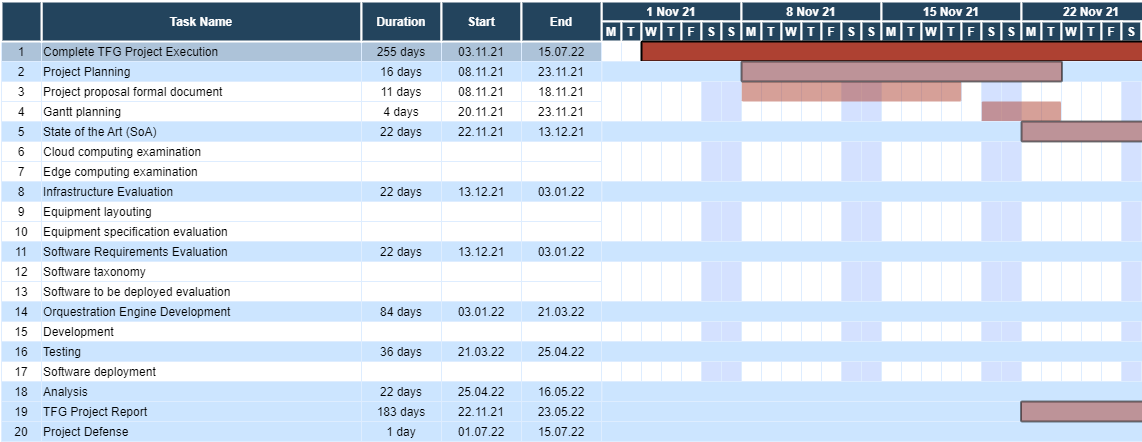
\includegraphics[width=\linewidth]{Images/gantt planning.png}
            \caption{Gantt diagram senior thesis planning}
            \label{fig:gantt}
        \end{figure}
    
        The technical part of the project development was done under the Agile mindset \cite{agile_manifesto_manifesto_nodate} with the Scrum \cite{scrum_guides_scrum_nodate} and Kanban framework. The different development phases were encompassed into Sprints of 1 week.

        \begin{figure}[H]
            \centering
            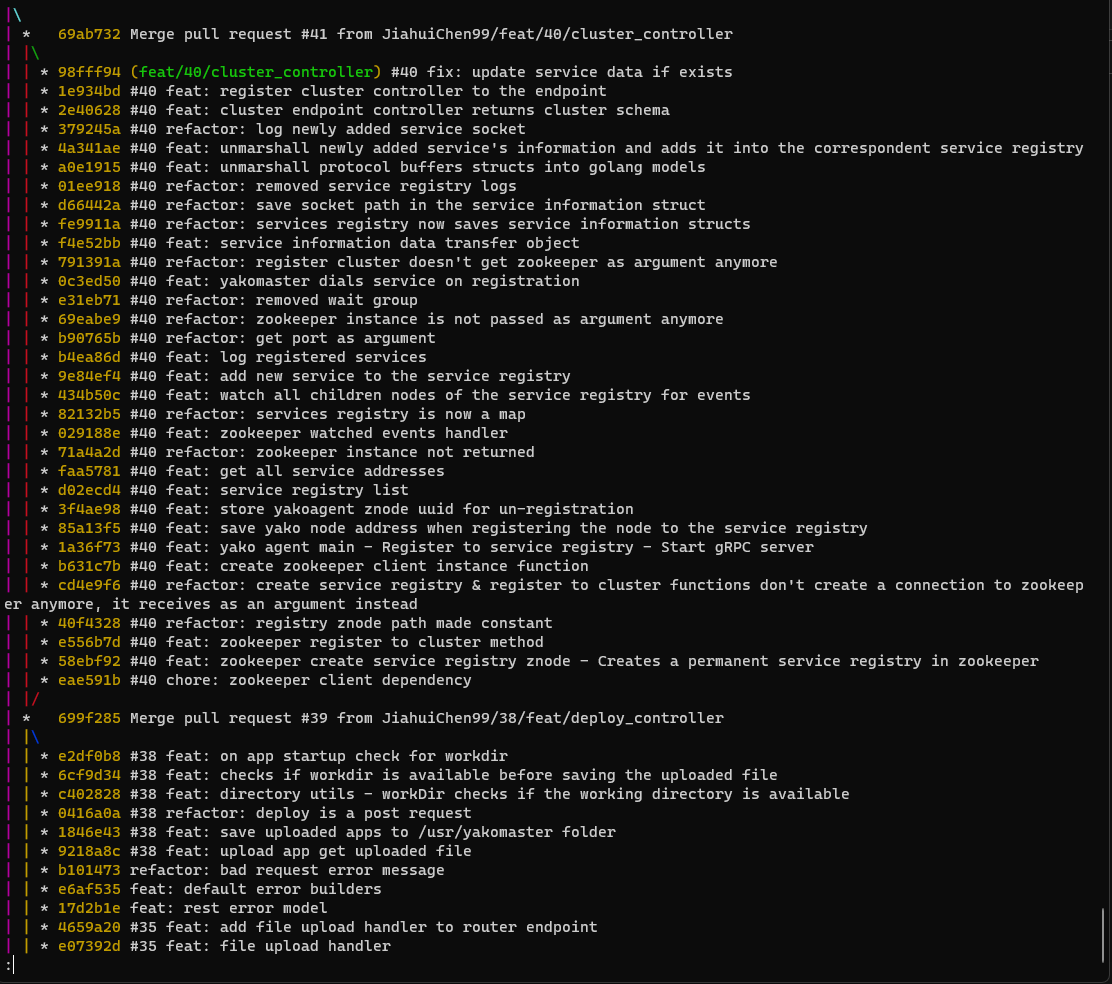
\includegraphics[width=0.6\linewidth]{Images/branches.png}
            \caption{Yako orchestrator back-end development Git log (branches, issues and commits)}
            \label{fig:branches}
        \end{figure}
        
        All the developed features were broken down into Stories and further separated into Technical Tasks, these are known as Issues on GitHub and were assigned with an ID and feature branch.
        During the development of the project, all the coded features were given its own branch and merged into the development(stable) branch after its implementation. The final release of the MVP is tagged to the main branch. Other best practices techniques, such as atomic commits \ref{fig:branches}, commits naming \cite{conventional_commits_conventional_nodate}, and broad documentation of the software were adopted.
        
        A total of 22 sprints with more than 100 GitHub issues \cite{chen_yako_2022-1} were produced.
        
        \begin{figure}[H]
            \begin{subfigure}{\textwidth}
                \centering
                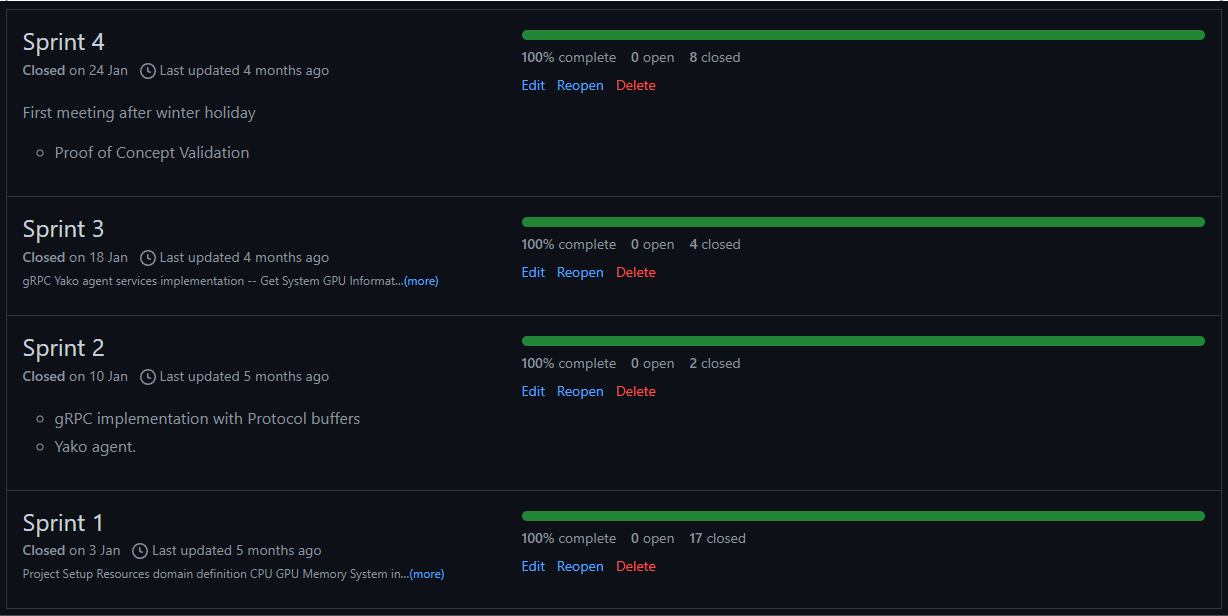
\includegraphics[width=0.8\linewidth]{Images/Sprints.png}
                \caption{Project Scrum Sprints}
                \label{fig:sprints}
            \end{subfigure}
            \begin{subfigure}{\textwidth}
                \centering
                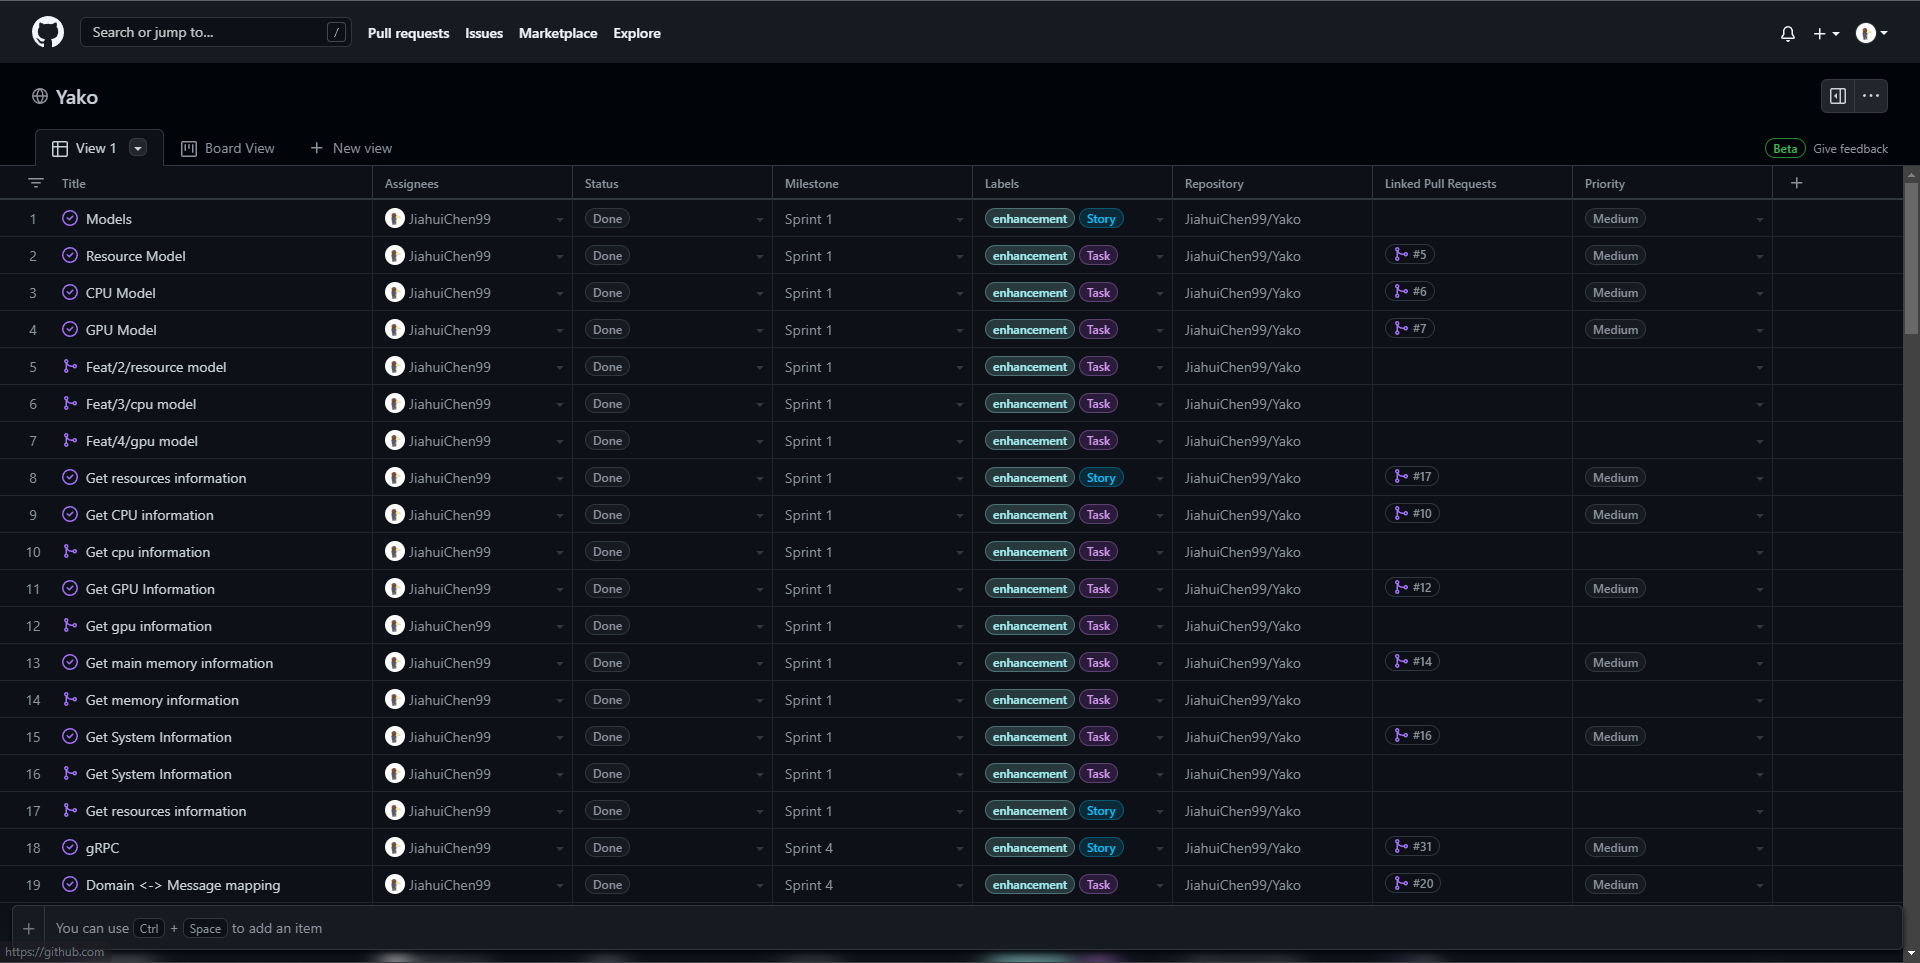
\includegraphics[width=0.8\linewidth]{Images/Issues.png}
                \caption{Yako project GitHub issues}
                \label{fig:issues}
            \end{subfigure}
            \caption{Scrum and Agile for Yako platform development}
            \label{fig:scrum}
        \end{figure}